\section{Poisson and the Birth of Potential Theory}

\subsection{From Laplace to Poisson: Sources Enter the Field}

By the early 19\textsuperscript{th} century, Laplace had given the mathematical form for fields in empty space. For a scalar potential \(\phi\), Laplace's formula expressed the balance of curvature:

\[
\frac{\partial^2 \phi}{\partial x^2} 
+ \frac{\partial^2 \phi}{\partial y^2} 
+ \frac{\partial^2 \phi}{\partial z^2} 
= 0.
\]

This described how quantities such as gravity or electrostatic potential varied smoothly in regions without any matter. But nature is rarely empty.

Siméon Denis Poisson recognized that this equation could not account for the presence of actual material bodies generating the field. He introduced a generalization by incorporating the density of matter, denoted \(\rho(x,y,z)\), directly into the equation:

\[
\frac{\partial^2 \phi}{\partial x^2} 
+ \frac{\partial^2 \phi}{\partial y^2} 
+ \frac{\partial^2 \phi}{\partial z^2} 
= - 4\pi \rho(x,y,z).
\]

This formula became known as \textbf{Poisson’s equation}. It completed the picture: matter no longer simply responded to existing fields — it created them.

\begin{HistoricalSidebar}{Potential Theory and the Machinery of Empire}

In the early 19th century, science in France was not simply a search for truth — it was a tool of state-building. 
After the Revolution, Napoleon reorganized French scientific institutions to serve the needs of empire: precision 
in artillery, navigation, geodesy, and infrastructure. Mathematics became a core instrument of imperial power.

\medskip

This is the world Poisson entered. His work on gravitation, elasticity, and electrostatics — formalized in what 
we now call the Poisson equation — was not pursued in isolation. Accurate gravitational models improved map-making 
and geodetic surveys, which were essential for tax collection, military planning, and colonial administration. 
Celestial mechanics refined navigation at sea, critical for controlling trade routes and projecting naval power.

\medskip

The institutions that supported Poisson — the École Polytechnique, the Bureau des Longitudes, the Académie 
des Sciences — were staffed by scientists who were simultaneously state bureaucrats. They were tasked not only 
with developing theory, but with producing tables, standards, and algorithms that directly served French 
geopolitical ambitions.

\medskip

Potential theory flourished in this ecosystem because it addressed exactly the kind of continuous fields — 
gravity, electric forces, fluid flows — that mattered for both cosmological understanding and practical 
statecraft. As Poisson extended Newton’s gravitational work into the language of partial differential equations, 
he was also extending the state’s ability to measure, predict, and control its expanding domain.

\medskip

While Poisson faced no religious opposition, he operated within a far more subtle political structure: a centralized 
academic-military-industrial complex, where success required both scientific brilliance and institutional alignment 
with the empire’s needs.

\begin{figure}[H]
    \centering
    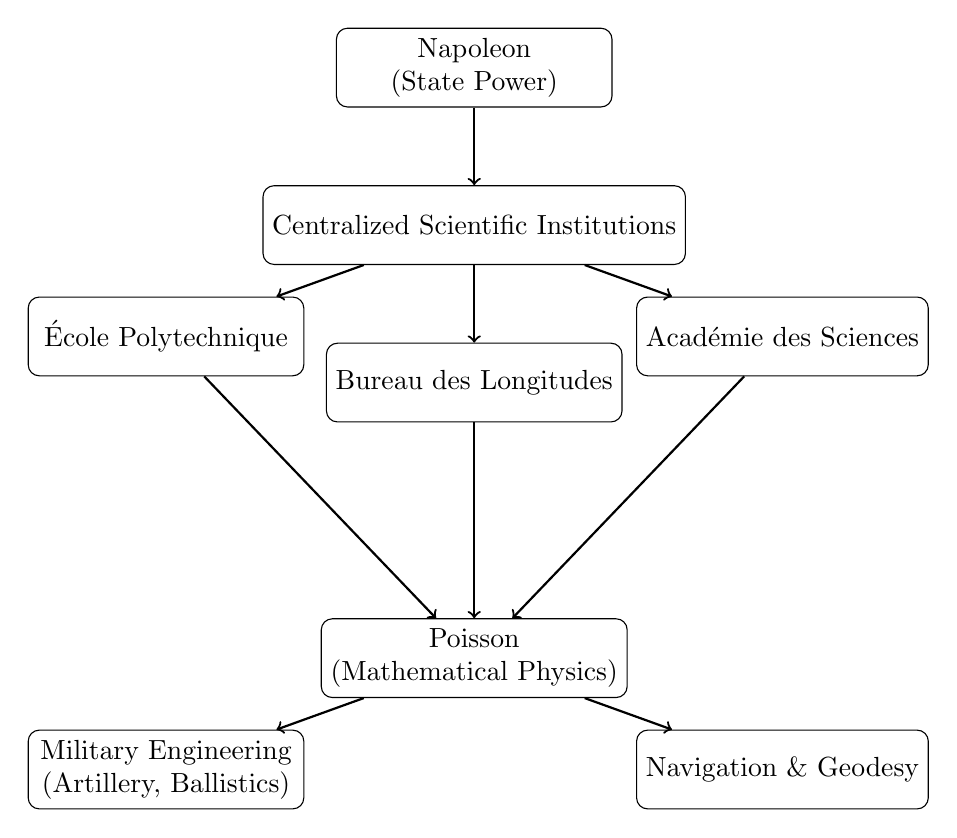
\begin{tikzpicture}[
      node distance=2cm,
      every node/.style={rectangle, draw=black, rounded corners, align=center, minimum width=3.5cm, minimum height=1cm},
      arrow/.style={->, thick}
    ]
    
    % Top Level
    \node (napoleon) {Napoleon \\ (State Power)};
    \node (institutions) [below of=napoleon] {Centralized Scientific Institutions};
    
    % Mid Level Institutions
    \node (polytech) [below left of=institutions, xshift=-2.5cm] {École Polytechnique};
    \node (longitudes) [below of=institutions] {Bureau des Longitudes};
    \node (academie) [below right of=institutions, xshift=2.5cm] {Académie des Sciences};
    
    % Poisson
    \node (poisson) [below of=longitudes, yshift=-1.5cm] {Poisson \\ (Mathematical Physics)};
    
    % Applications
    \node (military) [below left of=poisson, xshift=-2.5cm] {Military Engineering \\ (Artillery, Ballistics)};
    \node (navigation) [below right of=poisson, xshift=2.5cm] {Navigation \& Geodesy};
    
    % Arrows
    \draw[arrow] (napoleon) -- (institutions);
    \draw[arrow] (institutions) -- (polytech);
    \draw[arrow] (institutions) -- (longitudes);
    \draw[arrow] (institutions) -- (academie);
    \draw[arrow] (polytech) -- (poisson);
    \draw[arrow] (longitudes) -- (poisson);
    \draw[arrow] (academie) -- (poisson);
    \draw[arrow] (poisson) -- (military);
    \draw[arrow] (poisson) -- (navigation);
    
\end{tikzpicture}
    \caption{Institutional Power Map: Poisson’s Position in Napoleonic Science}
    \end{figure}

\end{HistoricalSidebar}


\subsection{The Integral Solution: Newton’s Law Reinterpreted}

For systems where the matter distribution \(\rho(x,y,z)\) is known, Poisson showed that the corresponding potential \(\phi\) can be calculated directly by summing the contributions of each infinitesimal portion of matter. The potential at a point \(P\) is given by the integral:

\[
\phi(P) 
= - \frac{1}{4\pi} \iiint \frac{ \rho(x,y,z) }{ R } \, dx\,dy\,dz,
\]

where \(R\) is the distance between the source point \((x,y,z)\) and the field point \(P\). That is,

\[
R = \sqrt{ (x - X)^2 + (y - Y)^2 + (z - Z)^2 },
\]

where \((X,Y,Z)\) are the coordinates of the observation point \(P\).

\medskip

This expression generalizes Newton’s formula for gravitational attraction from point masses to continuous bodies. Every element of matter contributes to the potential at \(P\), with strength decreasing inversely with distance.

\subsection{Spheres, Spheroids, and Ellipsoids: Poisson's Memoirs}

Poisson's work was not limited to simple geometries. In two important memoirs:

\begin{itemize}
    \item \emph{Sur l'attraction des sphéroïdes} (1829),
    \item \emph{Sur l'attraction d'un ellipsoïde homogène} (1835),
\end{itemize}

he extended potential theory to describe the attraction exerted by bodies shaped like flattened spheroids and ellipsoids. This allowed for more accurate models of planetary figures, tides, and astronomical perturbations.

\medskip

Laplace’s original formula worked only in empty space. Poisson’s generalization recognized that:

\[
\begin{cases}
\frac{\partial^2 \phi}{\partial x^2} 
+ \frac{\partial^2 \phi}{\partial y^2} 
+ \frac{\partial^2 \phi}{\partial z^2} 
= - 4\pi \rho(x,y,z) & \text{inside matter}, \\
\\
\frac{\partial^2 \phi}{\partial x^2} 
+ \frac{\partial^2 \phi}{\partial y^2} 
+ \frac{\partial^2 \phi}{\partial z^2} 
= 0 & \text{outside matter}.
\end{cases}
\]

In this way, the field distinguished between empty regions and material bodies.

\subsection{The Conceptual Shift: From Forces to Potentials}

Poisson’s approach also reflected a deeper philosophical transition in physics. Rather than calculating forces directly between particles, one could compute the potential \(\phi\), from which forces could be derived by differentiation:

\[
F_x = - \frac{\partial \phi}{\partial x}, \qquad
F_y = - \frac{\partial \phi}{\partial y}, \qquad
F_z = - \frac{\partial \phi}{\partial z}.
\]

Thus, the problem of gravitational attraction became one of calculating potentials — a major simplification when dealing with extended bodies.

\begin{HistoricalSidebar}{Poisson: Extending Newton by Way of Laplace}

Siméon Denis Poisson (1781–1840) stood at the intersection of Newtonian mechanics, Laplace’s celestial theory, and the emerging language of fields. As a student of both Lagrange and Laplace, Poisson became one of France’s leading mathematical physicists. His early work on electricity, magnetism, and mechanics introduced the systematic use of potentials as intermediaries between matter and force.

Poisson’s equation remains fundamental today not only in gravitation, but also in electrostatics, magnetism, and fluid dynamics. In every case, the same principle holds: \emph{matter creates curvature in the potential}.

\end{HistoricalSidebar}


\begin{HistoricalSidebar}{From Empirical Law to Field Equation: The Evolution of Gravity}

    When Newton formulated his famous law of universal gravitation,
    
    \[
    F = G \frac{m_1 m_2}{d^2},
    \]
    
    he presented it as an empirical rule—a precise summary of astronomical observations, but not derived 
    from more basic theoretical principles. It worked astonishingly well, but offered little hint of why 
    gravity behaved this way.

    \medskip
    
    By the early 19\textsuperscript{th} century, physicists like Laplace and Poisson began to reframe the 
    problem in terms of fields and potentials. Rather than imagining gravity as a mysterious force acting 
    instantly across space, they described it through a scalar potential \(\phi\), which varied smoothly 
    across space. Laplace’s equation applied in empty space; Poisson’s refinement introduced matter 
    density \(\rho\) as the source:
    
    \[
    \nabla^2 \phi = 4\pi G \rho.
    \]
    
    In this formulation, Newton’s inverse-square law emerged as a special solution (the so-called Green’s 
    function) to Poisson’s equation for isolated point masses. The gravitational force could now be 
    seen as arising from the spatial gradient of a potential field.

    \medskip
    
    This shift also hinted at a deeper structure: Poisson’s equation itself can be derived from a 
    variational principle. The Lagrangian density for Newtonian gravity takes the form:
    
    \[
    L = \frac{1}{8\pi G} (\nabla \phi)^2 + L_M,
    \]
    
    where \(L_M\) encodes the distribution of matter, with \(\delta L_M / \delta \phi = \rho\).

    \medskip
    
    Here, gravity is no longer just an empirical fact—it becomes a field theory derived from extremizing 
    an action. This approach foreshadowed the grand unifications of the 20\textsuperscript{th} century, 
    where forces emerge from variational principles and symmetries, much like the axiomatic structures 
    of mathematics.
    
    \medskip
    
    In this growing hierarchy, Newton’s formula stands to Poisson’s equation as Euclidean geometry stands 
    to Riemann’s manifold: a special case of a far more general framework.

    \medskip
\end{HistoricalSidebar}
